% !TeX encoding = UTF-8

\section{Fundamentals}

For preprocessing the images, a combination of methods are used: \textit{Image
Morphology}, \textit{Thresholding}, \textit{Contrast Limited Adaptive Histogram
Equalization (CLAHE)} and \textit{Masks}. These algorithms are provided by the
Python distribution of the Open Source library OpenCV \cite{opencv_library}.

\subsection{Definitions}

We define an Image $I$ with width $w$ and height $h$ to be the set
$I = \{ p_{xy} | x \in 1 \dots w, y \in 1 \dots h \}$. A RGB Image $I$ is an
Image with $p_{xy} \in (r_{xy}, g_{xy}, b_{xy})$, while a Greyscale image is
an Image with $p_{xy} \in 0,1, \dots 255$.

A Binary Image $B$ is an Image with $p_{xy} \in \{0,1\}$ where we also refer to
$0$ as \textit{black} and $1$ as \textit{white}

\subsection{Image Morphology}

Image Morphology is based on Mathematical Morphology from the mathematical field
of set theory. We are going to present two basic morphological operators
commonly used in image processing without going into detail of their
mathematical definition. A more formal definition and further reading can be
found in Aguardo (2012) \cite{Aguardo2012}

Given a binary image $B$ and a smaller binary image $B_s$ called the
\textit{Structuring Element}, we can apply the basic operations \textit{Erosion}
and \textit{Dilation}.

The Erosion $B \ominus B_s$ is equivalent to iterating through all of the white
pixels of $B$ and only keeping them if all of the points of $B_s$ translated
by its center point $c \in B_s$ to this position are fully included in $B$.
Therefore the white areas in $B$ are reduced . \cite{Smith1997}

Similarly for the Dilation operation  $B \oplus B_s$ , the Structuring Element
is translated to every pixel $p \in B$. For each of these pixels all the
neighbouring pixels that intersect with the translated $B_s$ are turned white.
The total area of white pixels is increased. \cite{Smith1997}

Image Morphologies have multiple uses like increasing certain areas for better
recognition or separating larger shapes of an image. In our case they will be
helpful for correcting interruptions in the black lines of the image as well as
for separating black areas that are bigger than typical lines.

% TODO: Possibly try to use Opening operation again and explain it here

\subsection{Concept}

%TODO: Define mondrian paintings in our context

Our aim for the detection algorithm is to take a cropped Mondrian painting as
an input and detect all the rectangles in it as well as their colors.

The input to algorithm is an RGB Image $I_1$ of a Mondrian painting. The
expected output is a list of rectangles with their position, sizes and color as
they are conceptionally seen in the painting. All rectangles combined are
expected to exactly cover the area of the input image in a way that the original
could be dissected into this set of rectangles. The thick black lines in the
paintings are seen as one-dimensional lines that are positioned in the middle
of the detected thicker lines.

The algorithm itself can be separated into two different phases: Image
preprocessing (\ref{preprocessing}) and the recognition of rectangles (\ref{rectangles}).

The goal of the first preprocessing phase is to obtain a binary image (an image
with only black and white pixels) in which black represent the lines of the
painting while white represents the inner area of the rectangles.

The second phase then takes this binary image and returns a list of found
rectangles. Additionally, for recognizing the colors of the rectangles, the
original input image is used.

\subsubsection{Image preprocessing} \label{preprocessing}

\begin{figure}
  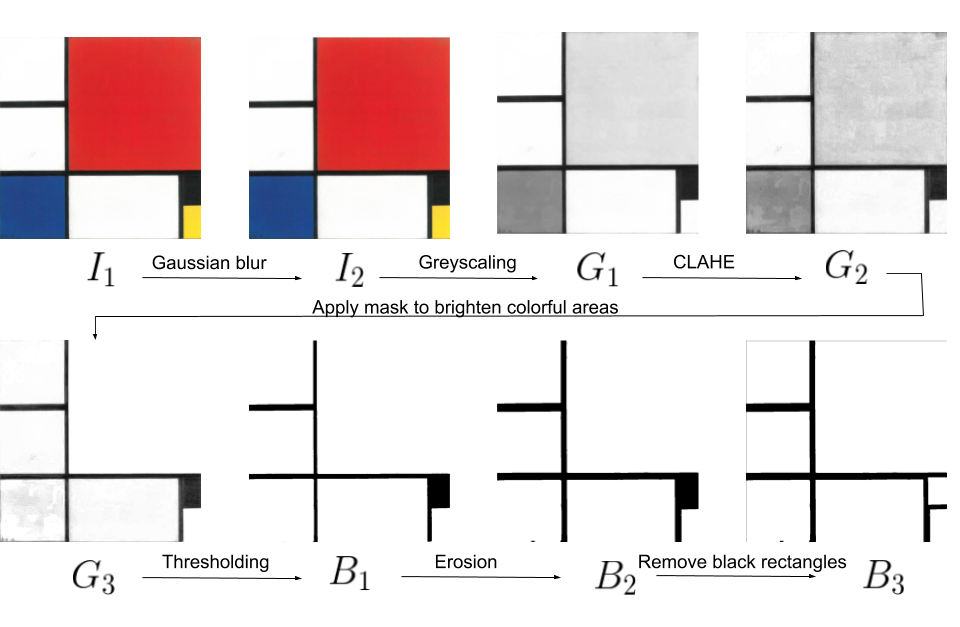
\includegraphics[width=\linewidth]{preprocessing_steps.png}
  \caption{Preprocessing Steps}
  \label{fig:preprocessing}
\end{figure}

At first, a Gaussian blur is applied to the input RGB Image
$I_1$ to reduce artifacts that the input images might include: $I_2 = G(I_1)$.
These artifacts might be craquelure or fading of darker areas in the paintings.
But they might also be results of the photography and scanning the images.

Next, the RGB input image is decomposed into a Greyscale Image $G_1$ by using
the maximum value of the RGB triplet for each pixel in $I_2$.

To normalize the lightness distribution of $G_1$ and increase the contrast of
the darker regions, we now apply histogram equalization to $G_1$. For this we
use \textit{Contrast Limited Adaptive Histogram Equalization (CLAHE)}. In
contrast to non-adaptive and ordinary adaptive histogram equalization
algorithms, this prevents the overamplification of noise. We call the result of
the equalization $G_2$. \cite{Pizer1987}

After the normalization is applied, we further brighten colorful areas of the
image to make them stand out against the black areas of the paintings. This way,
for example, darker blue areas can be better distinguished from black areas.
Since the difference between the maximum and the minimum value of the RGB
triplet is related to the colorfulness of a color, we calculate it for every
pixel of the input image. The resulting Mask $G_m$ from this calculation is added to
the contrast-normalized image $G_3 = G_2 + G_m$.

Now the image $G_3$ with the elements $g_{xy}$ is converted into a binary image
$B_1$ with the elements $t_{xy}$ using a threshold $t \in 0,1,\dots255$ for the
greyscale values. The value of $t$ needs to be chosen as such as its optimally
separating between the darker lines an the lighter rectangles in the image.

\begin{equation}
  t_{xy} =
  \begin{cases}
    0 & \quad  \text{if}  \quad g_{xy} \leq t\\
    1  & \quad \text{if}  \quad g_{xy} > t
  \end{cases}
\end{equation}

% TODO: How is N choosen? Why can it result in loss of information?

Since the thresholding step might leave some interruption in the black lines, we
reduce the white areas of the image: An Erosion $B_2 = B_1 \ominus B_e$ is
applied. In this case, the structuring element $B_e$ is a $N\times N$ binary
Image. Using the Erosion some accidental interruptions in the lines can be
restored. However choosing a the Structuring Element that is too high, might
result in loss of information. Therefore the size $N$ needs to be chosen
carefully.

The resulting image $B_2$ now separates the darker parts of the image fairly
well. However, we are only interested in black lines, but Mondrian paintings
also include filled black rectangles. To remove these black rectangles, we
create a mask that applies a Dilation $B_m = B_2 \oplus B_d$ with a larger
Structuring Element $B_d$ compared with $B_e$ on the image. The size of $B_d$ is
chosen in a way that most of the lines in the paintings are removed, only
leaving inner areas of black rectangles. The resulting mask $B_m$ is then
removed from the image of the last step $B_3 = B_2 - B_m$. Hence only the
outlines of the black rectangles, as well as the black lines, remain in $B_3$.

%TODO(29): Create an image showing the preprocessing steps

\subsubsection{Detection and recognition of rectangles} \label{rectangles}

Since the rectangles in the input image are defined by the horizontal and
vertical lines in the image, the detection starts by finding all of those lines
in the output binary image from the previous phase.

%TODO: Explain Horizontal vs. Vertical better

To find horizontal lines, the image is scanned line by line for each pixel.
Uninterrupted sequences of black pixels are added to a list of horizontal lines.
Only sequences with a specified minimum length are added. The minimum length
should ideally be slightly larger than the maximum width of the lines in the
image. Vertical lines are recognized respectively. This step is the equivalent of
applying a lossy run-length encoding once horizontally and once vertically.

However, this means that what we perceive as one horizontal line in the painting
is now recognized as multiple lines next to each other. For example, a line that
is 50 pixels wide would be recognized as 50 lines. Therefore as a next step
parallel lines close to each other are merged into a single line. As long as
parallel lines are within a certain distance from each other, they are merged
into one line. For horizontal lines, the resulting line will have the average
$y$ value of all those lines and the minimum and maximum $x$ values as starting
and end points.

From out idealistic view on Mondrian paintings, the ends of lines always touch
another line or the edge of the painting. However, the lines that we reduced now
might overlap slightly or not even connect to the next line.

% TODO: Specify how to find the closest line

We, therefore, iterate over all the ends of the lines, determine the closest
line to this point and change the position of this end to the closest line. For
the purpose of this algorithm, the edges of the image are considered to be lines
as well.

%TODO: How are they identified as top-left?

All lines should now represent the structure of the painting. What we want as
our output though is a list of rectangles. Every rectangle in the image can be
defined through a set of four different corners: top-left, top-right,
bottom-left and bottom-right. These corners are always intersections of two
lines, either crossing or touching. We determine the corners and their types by
iterating through the lines.

After this, four different corners are combined into a rectangle by finding
matching corners. This is done by iterating through the top-left corners $(x,y)$
and finding the closest top-right corner to the right $(x_r, y)$ and the
closest bottom-left corner below $(x, y_b)$. The rectangle is then defined by
the position of the top-left corner and its width and height
$(x,y,x_r-x,y_b-y)$.

For this list of rectangles, we determine the colors of the rectangles. For this
purpose, we clip the rectangle from the original image and determine the average
color or the selection. This color is then reduced to either black, white, red,
blue or yellow.

\section{Implementation}

%TODO: Write implementation

Challenges?
Code: Pseudo/Python?
How do the choose threshold t?
Min length t?
Distance d?
How to choose N?

Thresholding:
Through test runs a value of 110 for a greyscale range of 0 to 255
showed to give the reasonable results.
